\chapter{SURVEY DESIGN AND METHODS}
\section{Survey Study of Michigan Inland Lakes} 
As a grantee of \gls{mdeq}, our main objective is to develop a predictive model. We address the challenge by assessing land use information and collected cyanotoxin data and investigate statistical relationship that potentially drives \gls{hab}. For the summer of 2017, a total of 29 inland lakes were sampled. Prior to sampling, permission of riparian owner was obtained for lakes which did not have public access. Sample surveying began in the month of June 2017 until October 2017. Each month, every lake one was sampled once. Sampling locations were chosen from known list of lakes reported with \gls{hab} given by Aaron Parker from \gls{mdeq} and existing collaborative partners with different lake associations. In addition, we also chose lakes that are reasonably close to I-75 expressway for the ease of transportation. See figure \ref{fig:overview} for a map of our lakes sites and for more detail, see table \ref{tab:Surveyed Lakes}.

Cyanotoxins were analyzed primarily by \gls{lcmsms}. For \gls{mc}, 12 different congeners along with nodularin were identified and quantified by \gls{lcmsms}. Total \gls{mc} is the sum of the 12 congeners and nodularin analyzed by \gls{lcmsms} measured in the sample. In parallel, \gls{elisa} was used to quantify total \gls{mc} and nodularins.  we compared the results of total \gls{mc} from both \gls{lcmsms} and \gls{elisa} and assessed the agreement between the two. Cylindrospermopsin and Anatoxin-a were also analyzed with \gls{lcmsms}. In addition, we also used \gls{qpcr} which detects and quantifies \emph{16s rRNA}, \emph{mcyE/nadF}, \emph{sxtA}, and \emph{cyrA} gene. The \emph{16s rRNA} gene is a common gene in \gls{qpcr} to uniquely identify bacterial phylogeny and taxonomy \cite{janda_16s_2007}.  The \emph{mcyE/nadF}, \emph{sxtA} and \emph{cyrA} are gene clusters responsible of synthesizing \gls{mc}, nodularin, saxitoxin-a and cylindrospermonsin. A commercial kit from Phytoxigene Inc. \footnote{Phytoxigene Inc. Diagnostic Technology, 7 Narabang Way, Belrose 2085. Australia.} is used for \gls{qpcr} which contains the neccessary primers and probes.  

At the beginning of our survey, a constructed sampler string was installed at each lake. The sampler was constructed by the Dr. Raffel's team, which consisted of 3 gray PVC plates and placed at each sampling location for the purpose of collecting zebra mussels (see figure \ref{fig:samplerr}). The stack of three square PVC plates were  15 cm,20 cm, and 25 cm in diameter which gives them a total surface area of 0.23 m$^2$ per sampler. In addition, each sampler string included a slotted PVC pipe, seperated into two halves and capped on either end to hold SPATT. This was a beta test of a new method for monitoring toxins. Sampler strings were either hung beneath riparian owner's dock or from a labeled float, with the SPATT samplers and zebra mussel samplers suspended aproximately 20 cm and 30 cm below the surface, respectively. HOBO\texttrademark pendant temperature and light loggers were attached to the sampling string at the level of the SPATT sampler. In October, we collected the samplers and scraped all mussels into a glass mason jar for analysis of biomass, after the juvenile mussel settlement (August to September) had ended.

We analyzed different water parameters we hypothesized should lead be key drivers of \gls{hab}. Upon arrival at each lake we measured pH, conductance and dissolved oxygen. A portable nephelometer and flurometer was used to measure turbidity, chloraphyl-a and phycocyanin. Dissolved nitrate+nitrite, orthophosphate, ammonia, total phosphorus and nitrogen were analyzed colorimetrically on the collected water samples. Land use for each lake's watershed was calculated using \gls{gis} software. Data was compiled for statistical analysis.

\begin{figure}[!h]
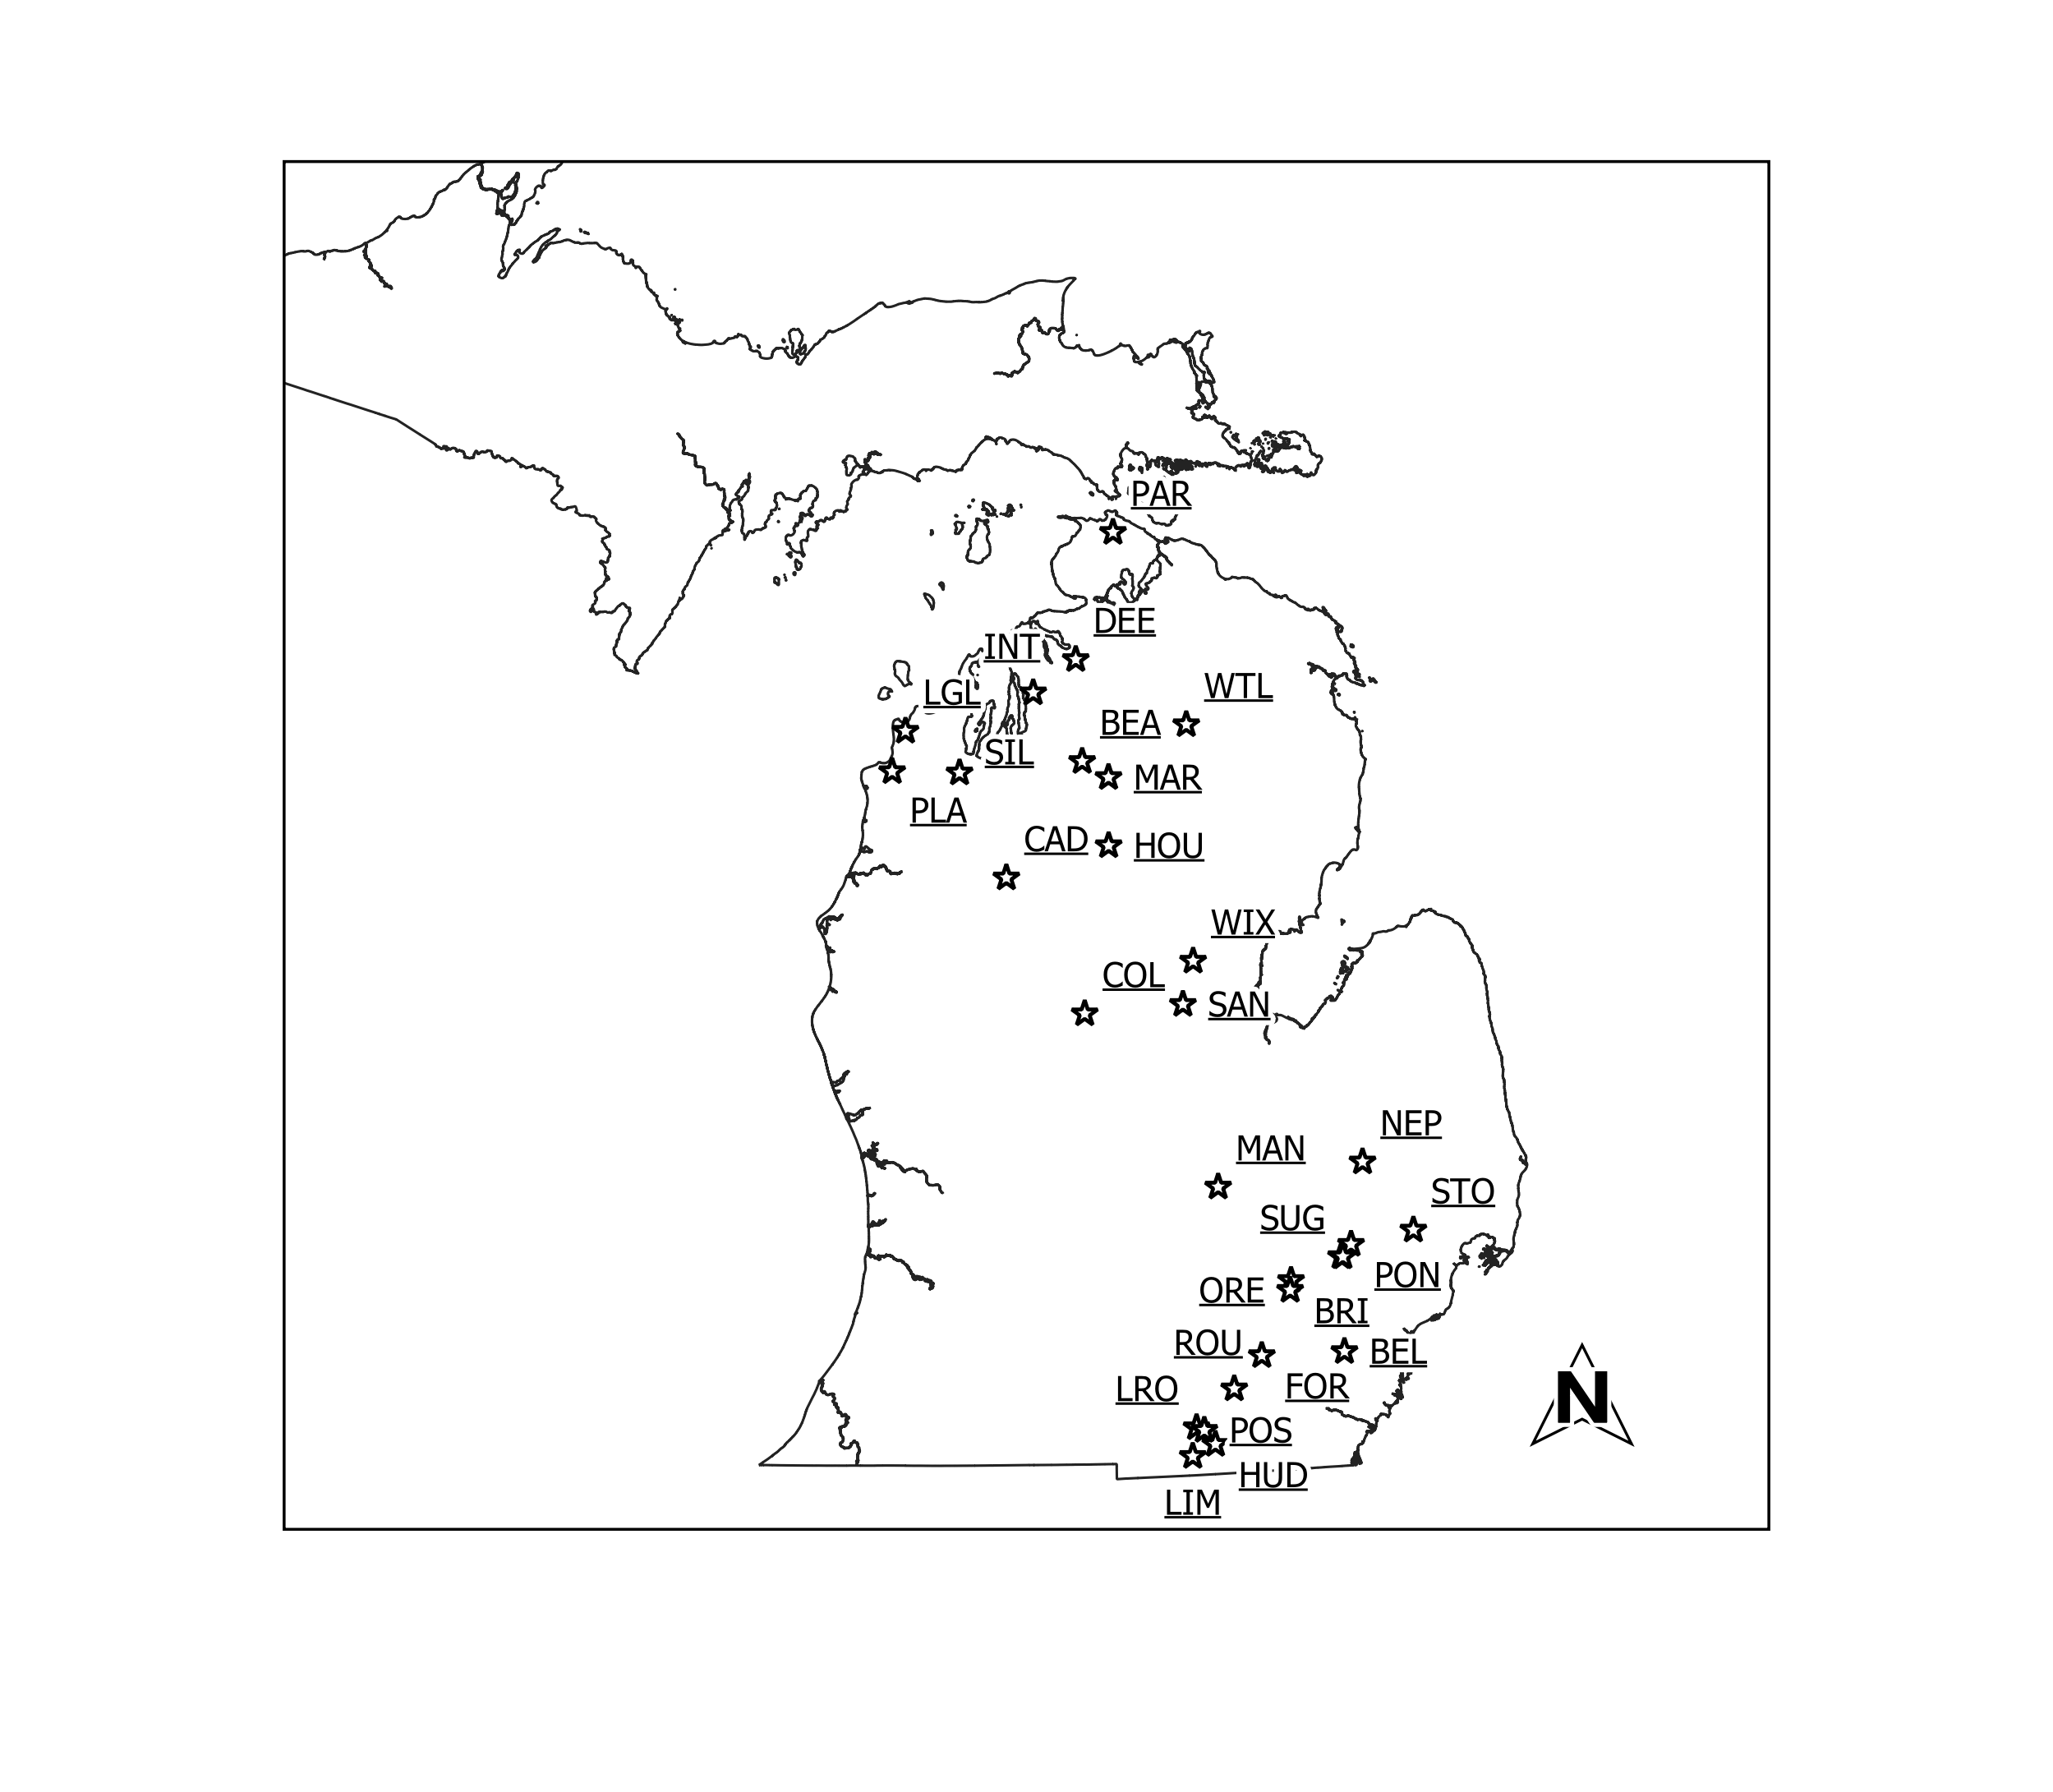
\includegraphics[width=\textwidth]{figures/Overview}
\caption{Map of Sampled Lake Sites in Michigan.}
\label{fig:overview}
\end{figure}

\begin{sidewaystable}
\caption{Geographic information of sampling points at each  surveyed lakes. }
\label{tab:Surveyed Lakes}
\begin{center}
\scalebox{0.86}{
\begin{tabular}{lllrrl}
\hline \\
\multicolumn{1}{c}{Name of Lake} & \multicolumn{1}{c}{Shorten Code} & \multicolumn{1}{c}{County} & \multicolumn{1}{c}{Longitude} & \multicolumn{1}{c}{Latitude} &
\multicolumn{1}{c}{HUC 14 Reachcode} \\ \hline
Bear Lake & BEA & Kalkaska & -84.9438079727 & 44.7286139551 & 04060103001048 \\
Belleville Lake & BEL & Wayne & -83.4663770506 & 42.2145253455 & 04090005001822 \\
Bogie Lake & BOG & Oakland & -83.5054334514 & 42.6188513679 & 04090005001348 \\
Brighton Lake & BRI & Livingston & -83.7958137995 & 42.5169054061 & 04090005001500 \\
Coldwater Lake & COL & Isabella & -84.9565922285 & 43.6613607551 & 04080202000902 \\
Deer Lake & DEE & Charlevoix & -84.9770123186 & 45.166441811 & 04060105001116 \\
Ford Lake & FOR & Washtenaw & -83.5849122567 & 42.2159133043 & 04090005001823 \\
Houghton Lake & HOU & Roscommon & -84.7262816343 & 44.3385407778 & 04060102002461 \\
Hudson Lake & HUD & Lenawee & -84.2545514803 & 41.835000535 & 04100002001317 \\
Intermediate lake & INT & Antrim & -85.2293359783 & 45.0265435299 & 04060105003435 \\
Lake Cadillac & CAD & Wexford & -85.4266252378 & 44.2410192547 & 04060102001951 \\
Lake Margrethe & MAR & Crawford & -84.7830175986 & 44.6464747348 & 04060103001058 \\
Lake Nepessing & NEP & Lapeer & -83.3728265865 & 43.0161554865 & 04080204001601 \\
Lime Lake & LIM & Hillsdale & -84.3791188315 & 41.7861576065 & 04100006000872 \\
Little Glen Lake & LGL & Leelanac & -85.963633169 & 44.8687577197 & 04060104000456 \\
Little Round Lake & LRO & Lenawee & -84.3527742524 & 41.9093334799 & 04100006000858 \\
Manitou Lake & MAN & Shiawassee & -84.2038069227 & 42.925537136 & 04050005000939 \\
Ore Lake & ORE & Livingston & -83.7959940227 & 42.4805569493 & 04090005001574 \\
Paradise Lake & PAR & Emmett & -84.7512093045 & 45.6872890124 & 04060105001063 \\
Platte Lake & PLA & Benzie & -86.092789204 & 44.6900468421 & 04060104000558 \\
Pontiac Lake & PON & Oakland & -83.451096479 & 42.6664394508 & 04090005001288 \\
Posey lake & POS & Lenawee & -84.3007962072 & 41.8970465491 & 04100006000857 \\
Round Lake & ROU & Lenawee & -84.1318219224 & 42.0712488438 & 04100002001130 \\
Sanford Lake & SAN & Midland & -84.3860517762 & 43.7104273774 & 04080201001468 \\
Silver Lake & SIL & Grand Traverse & -85.687150728 & 44.6980286859 & 04060105003542 \\
Stony Creek Lake & STO & Oakland & -83.0870627175 & 42.7260717429 & 04090003001029 \\
Sugden Lake & SUG & Oakland & -83.4972563639 & 42.6173106359 & 04090005001347 \\
West Twin Lake & WTL & Montmorency & -84.3501403918 & 44.8762035424 & 04070007001271 \\
Wixom Lake & WIX & Gladwin & -84.3537506311 & 43.8276751177 & 04080201001442 \\ \hline
\multicolumn{3}{r}{{HUC=Hydrological Unit Code}} \\ \hline
\multicolumn{3}{r}{{GPS Coordinates are in decimal degrees, North American Datum of 1983 (NAD83)}} \\ \hline
\end{tabular}}
\end{center}
\end{sidewaystable}


\begin{figure}[!h]
\centering
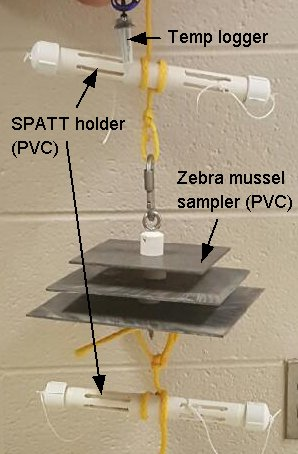
\includegraphics[width=\textwidth, height=18cm]{figures/samplers}
\caption{Picture of the constructed sampler installed at each lake. HOBO Pendant is attached with a secure carabiner. SPATT PVC holders and Zebra mussel sampler is shown.}
\label{fig:samplerr}
\end{figure}

\clearpage
\subsection{Water Sampling} \label{sampling}

Water samples were collected by wading in toward the center of the lake until water height reached waist height. All water grab samples were taken roughly one foot below water surface. Each water collecting vessel was rinsed 3 times with the lake water before obtaining final sample. A total of 4 teams of field surveyors sampled the designated lakes. At each lake, a hand-held multi-meter was used to measure pH, conductivity ($\mu$S/cm), dissolved oxygen (mg/L) and temperature ($^\circ$C). Phycocyanin and chlorophyll fluorescence were also measured using an portable fluorometer by Amiscience with the optical excitation of 470 nm and 590 nm and the emission is read at 685 nm, which is measured in \gls{rfu}. Each fluorometer for each surveyor was calibrated against rhodamine WT\footnote{Sodium chloride 4-[3,6-bis(diethylamino)-9-xantheniumyl]isophthalate (2:1:1)} dye as a secondary calibration standard, which ensured the calibration relative to other fluorometer and prevent drift. A portable meter from Hach was used to measure turbidity in \gls{ntu}. Formazin standards were used to calibrate the turbidity meter.

Water sampling kits were prepared by storing pre-labeled water vessels in zip-lock bags for each lake to prevent cross-contamination between different lake water samples during sampling transport and storage. Each sampling kit contained 60mL \gls{petg} vials for MC analysis, 100mL sterile IDEXX bottles for QPCR analysis, 50mL polypropylene centrifuge vials and 250 mL \gls{hpde} Nalgene bottles for nutrient analysis. Each kit also provided alkaline Lugol's iodine solution for preserving cyanobacteria samples for identification and 3M \ch{H2SO4} for acid preservation of nutrient samples. The 3M \ch{H2SO4} is in a separate zip-lock bag with roughly 20g of \ch{NaCO3} wrapped in paper towel to neutralize the sulfuric acid incase of a spill or a leak. Lugol's iodine solution was prepared by dissolving 100g of \ch{KI}, 100g of \ch{I2} and 100g of sodium acetate dissolved in 1 liter of water. See figure \ref{fig:samplekit} for an example of a sampling kit.

\begin{figure}[!h]
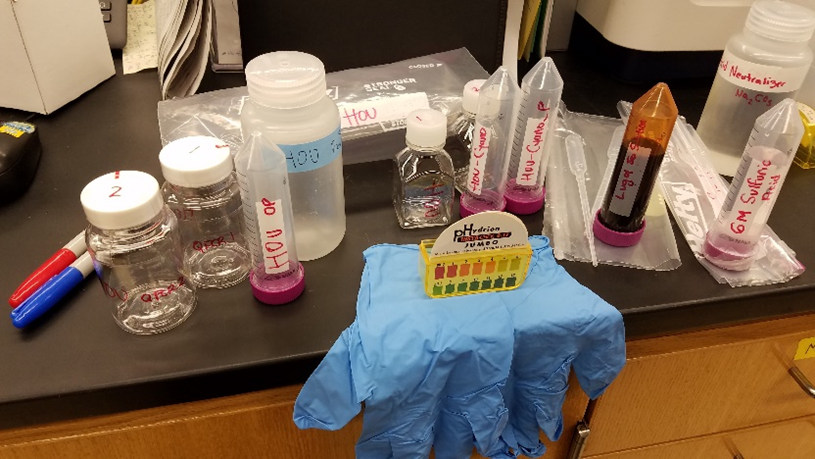
\includegraphics[width=\textwidth]{figures/samplekit}
\caption{An example of sampling kit and the contents}
\label{fig:samplekit}
\end{figure}

\clearpage
\newpage

\section{Analytical Methods}

\subsection{Liquid Chromatography Mass Spectrometry} \label{sc:lcms}

\paragraph{Grab Samples}

Water samples were collected in 60mL \gls{petg} vials upon arrival at each lake. Within 3 days from sampling, the water samples were freeze-thawed for 3 cycles for cell lysis. Water samples are thawed slowly in a heated water bath at 37$^\circ$C, then frozen at -20$^\circ$C. Once finally thawed, an AcroPrep 96-well plate with glass fiber was used to filter the water samples. Once filtered, a 3.5 mL aliquot of each sample was transferred to glass vials suitable for the Thermo Scientific EQuan MAX (online sample concentrator). The samples were transported to the Westrick group at Wayne State University and analyzed for 12 MC congeners, nodularin, anatoxin-a and cylindrospermopsin.  The Westrick group uses a a high-throughput \gls{lcmsms} analysis for \gls{mc} in surface and drinking water analyses.
The analysis done by the Westrick group's \gls{lcmsms} platform includes a Thermo Scientific EQuan MAX (online sample concentrator) and ThermoFisher’s UltiMate 3000 \gls{uhplc} system and a \gls{tsq} Quantiva.
Their method is similar to EPA method 544 with the addition of 5 more congener analytes \cite{shoemaker_method_2015}. Figure \ref{fig:spectra} shows a standard chromatogram of all 12 \gls{mc}, nodularin, and the ethylated internal standard (\ch{[C_2D_5]} MC-LR) eluting between 2.2 and 5.2 minutes allowing for the total analyses time to be less than 12 minutes.  The \gls{mdl} is 0.030  $\mu$g/L  for all cyantoxin analysis. 

\paragraph{Solid Phase Adsorption Toxin Tracking}

The SPATT bag is constructed with Nitex\footnote{Purchased from Dynamic Aqua-Supply Ltd.  \url{http://www.dynamicaqua.com/nitex.html}} and filled with Diaion\texttrademark \: HP-20\footnote{Purchased from Sigma Aldrich: CAS Number 9052-95-3}, a non-polar resin (styrene-divinylbenzene copolymer). To construct the SPATT bags, a 1 meter x 5 centimeter strip of Nitex mesh was cut with a sharp blade. The Nitex strip was sewn by folding half length-wise (or \emph{hot dog} style). With tape holding the fold, the end of the strip was sewn 0.5cm from the edge. The sewn end were stitched with a tight pattern done with a clear nylon thread to ensure no leakage of polymer beads. Approximately 9-10cm lengths of sewn Nitex tubes were cut and zip-tied about 0.5cm at one end. With one end open, 3.00-3.01 grams of HP-20 resin was carefully inserted using a funnel. The open end was zip-tied once the Nitex bag was full. Prior to deployment, the filled SPATT bags were activated by soaking in 100\% methanol for 24 hours under $4^\circ$C. Next the SPATTs were rinsed with Milli-Q water and then soaked for 24 hours in Milli-Q water under $4^\circ$C before deploying the SPATT bag in our target sample lakes.

At each lake site, two SPATT bags were loaded into the slotted PVC pipe on the constructed float. The SPATT bags were left for about a month at each lake. When SPATT were retrieved, they were carefully removed and rinsed with Milli-Q water upon arrival and stored in a 15mL centrifuge vial with a plastic spacer on the bottom. SPATT were stored at $4^\circ$C during transport back to the lab. The SPATT were centrifuged at 8000rpm. The spacer allows liquid to pool on the bottom when centrifuged. When centrifuged, the SPATT bags were cut open and the resin was poured into a 50mL centrifuge tube. Milli-Q water was used to rinse the SPATT bags to effectively transfer all the resin. About 30mL of Milli-Q water was used. The solution was allowed to rest so the resin settles to the bottom. Using a pipet, the water was carefully decanted until the total volume was 5mL.  A solution of 80\% methanol with 10$\mu$M ammonium formate was added to the tube until the total volume was 45mL. The solution was gently mixed and then allowed to settle for 30 minutes. A 3.5mL aliqout of the supernatant was transferred to glass vials and analyzed by \gls{lcmsms} by the Westrick group. Similiar to our analysis of the grab sample, the SPATTs were analyzed for all 12 congeners of \gls{mc} and nodularin. The final reported value was calculated to give the amount of \gls{mc} per gram of resin per day. It was calculated by this equation:

\begin {center} 
$(\frac{\text{ng of MC}}{\text{g of resin per day}}) =(\frac{\text{$\mu$g of MC}}{L}) \times (\frac{\text{1000ng}}{\text{$\mu$g}}) \times {0.045L} \times \frac{1}{\text{3g of resin}} \times \frac{1}{\text{days deployed}}$
\end{center}


\begin{figure}[!h]
\centering
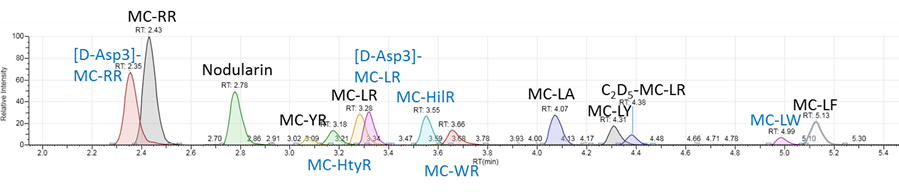
\includegraphics{LCMS_CONGENERS}
\caption{Liquid chromotography-mass spectrometry chromatogram of the MC congeners. Chromatogram provided by Westrick Group.}
\label{fig:spectra}
\end{figure}

\clearpage

\subsection{Enzyme-Linked Immunosorbant Assay}

A commercial Microcystin/Nodularins ADDA ELISA kit was used from Abraxis to analyze total microcystin\footnote{https://www.abraxiskits.com/products/algal-toxins/}. The analysis uses a polyclonal antibody which specifically binds to the ADDA moiety found in MC. However it does not distinguish between different congeners and the given results are provided in terms of MC-LR equivalence. The analysis followed the recommended guidelines provided by the EPA \cite{usepa_method_2016}. In preparation for loading the plate,  100 $\mu$L of standards, controls, blanks and samples are aliquoted into a separate sterile 96-well plate. To minimize assay drift caused by slow plate loading, a multi-channel pipettor was used to load the standards, controls, blanks and samples to the final 96-well plate. The assay procedures were carried out and read by a Synergy H1 microplate reader from Biotek.

\subsection{Quantitative Polymerase Chain Reaction}

Phytoxigene\texttrademark  CyanoDTec cyanobacteria and toxin \gls{qpcr} was performed with the Applied Biosystem StepOnePlus\texttrademark. The kit provides two separate assay mixes. The total cyanobacteria assay will quantify the \emph{16s rRNA} gene copies found in the water sample. The toxin kit will quantify the \emph{mcyE}, \emph{sxtA} and \emph{cyrA} gene copies.  Both the total cyanobacteria and toxin gene assay were analyzed in parallel for each month of grab samples. The primer/probe sequence is proprietary and unknown.  The PCR reaction mix contained 5 $\mu$L of template/sample extract and 20 $\mu$L of rehydrated mastermix.  Each sample was run in singlicate due to limited resources. Positive standards for target genes  were run on each PCR analysis. Phytoxigene\texttrademark  CyanoNAS nucleic standards were used to generate standard curves for quantification of gene copies. The CyanoNAS was removed from -20$^\circ$C and allowed to thaw prior to analysis.  Standards were run in duplicates.

Samples for QPCR were filtered either on site with a portable Santino pump, or brought back to the lab for filtration within 8 hours from sampling.
At each lake, 100mL or more of water sample was collected in a sterile IDEXX vessel then filtered through a 0.4 $\mu$m pore size polycarbonate membrane  and stored at -20$^\circ$C until QPCR. Once filtered, they are immediately transferred into BioGX vials. BioGX vials are stored at -80$^\circ$C until analysis. BioGx vials contains 500 uL of lysis buffer, lysis beads and filtrate. For cell lysis, vials were vigorously shaken by bead beater on the highest setting for 2 minutes. After bead beaten, sample vials were centrifuged for 1 min. After centrifuge, 50 $\mu$L of the supernatant was transferred to a microcentrifuge tube and centrifuged for 5 min, then roughly 25 $\mu$L of the final supernatant was transferred to another set of microcentrifuge tubes for PCR.  Sample extracts are stored at 4$^\circ$C and analyzed within 4 hours. Finally, 20 $\mu$L of hydrated mastermix and 5 $\mu$L of sample extracts is aliquoted into the PCR plate.

From following the recommended guide by Phytoxigene, the PCR heat cycles were programmed with an initial denaturing step at 95$^\circ$C for 2 min, then a repeating of 95$^\circ$C for 15 seconds and 60$^\circ$C for 30 seconds reaching a total of 40 cycles. The appropriate gene target filters were manually set to match the emission spectrum of each probe. For each PCR run, a standard curve was generated  from within the StepOnePlus software. CT threshold and baseline were manually assigned for each run by visually assessing each target run. The calculated gene copies were done automatically by the StepOnePlus software, expressed in gene copies/$\mu$L of lysate. The final reportable value was calculated by this equation:

\begin{center}
	$\frac{Genecopies}{mL} = (\frac{Genecopies}{\mu L \: of \: lysate}) \times (\frac{500\mu L \: of \: lysate}{\text{mL of Sample Volume}})$
\end{center}

\subsection{Nutrients}

Two 125-mL \gls{hpde} Nalgene bottles were used to collect acid-preserved water samples with 2 mL of 3M \ch{H2SO4}, resulting to pH \textless 2. A 50-mL centrifuge tube is used to collect water samples without acid preservation for orthophosphate. One of the two Nalgene bottles is allocated for ammonia-N and nitrate+nitrite-N by our lab at Oakland University, and the other is for total phosphorus and total nitrogen run by Ben Southwell and his team at Lake Superior State University.  Samples were kept  at 4 $^\circ$C during transport and stored at -20$^\circ$C. Upon receiving samples from field samplers samples are thawed if frozen and cool at 4$^\circ$C. All lake water samples were homogenized by inverting 8 times and aliquoted into 15-mL centrifuge vials and centrifuged at 3000rpm for 45 seconds. The supernatant was collected into a clean 3-mL vial to be prepared for the AQ1 auto sampler. All samples were analyzed within the appropriate time frame from time of sampling collection.

Nutrient concentrations are quantified by colorimetric analysis with  AQ1 from SEAL Analytical\footnote{SEAL Analytical Inc.
6501 West Donges Bay Road Mequon, Wisconsin 53092}.  Ammonia-N (\ch{NH3}) is quantified by a reaction with dichloroisocyanurate and dissolve ammonia to create chloramines which  forms a blue-green color with salicylate which is measured at 660 nm \cite{usepa_method_1993-2}. The range of application is between 0.02-1.0 mg N/L with a mininum detection limit of 0.006 mg N/L for quantifying ammonia.  Nitrate+nitrite-N (\ch{NO3^{-}} $+$ \ch{NO2^{-}}) is analyzed with an open tube copperized cadmium coil which the pH buffered sample water will have nitrate reduced to nitrite. The reduced water sample is then reacts with sulfanilamide with the presence of $N$-(1-napthyl)-ethylenediamine dihydrochloride to form a reddish color measured at 520 nm \cite{usepa_method_1993}. The range of application for analyzing nitrate+nitrite is between 0.25-15 mg N/L with a detection limit of 0.04 mg N/L.  Orthophosphate-P (\ch{PO4^{-3}}) is analyzed with acidic molybdate solution with antimony potassium tartrate to form a complex with dissolved orthophosphate. The complex is reduced with ascorbic acid to create a blue color measured at 880 nm \cite{usepa_method_1993-3}. The range for orthosphosphate is between 0.003-0.3 mg P/L with 0.008 mg P/L as the detection limit. Total Kjeldahl nitrogen-N (organic nitrogen) is analyzed by sample digestion with copper(II) catalyst at 380$^\circ$C. Nitrogen containing compounds such as amino acids and peptides are converted to ammonia which is then reacted with hypochorite to create chloramine, which is then reacted with salicylate at a pH of 12.6 with the presence of nitroferricyanide to form a green-blue color measured at 670 nm \cite{usepa_method_1993-1}. The range for total Kjeldahl nitrogen is between 0.2 to 4.0 mg N/L with 0.07 mg N/L as the detection limit. Total phosphorus (polyphosphates and some organic phosphorus)  is analyzed by acid-persulfate digestion which water sample with ammonium persulfate and sulfuric acid is autoclaved at 121$^\circ$C for 30 minutes which organic phosphorus is converted to orthophosphate. After digestion, orthophosphate is reacted with acidic molybdate which is reduced by ascorbic acid to create a blue color measured at 880 nm \cite{usepa_method_1993-3}. The range for total phosphorus is between 0.01-1.0 mg P/L with 0.02 mg P/L as the detection limit. 


\subsection{Geographic Information System Analysis}

Watershed delineation and calculation of land use were done using \gls{qgis} \cite{qgis_development_team_qgis_2009}.
Elevation data was downloaded in bulk by an FTP client as mosaic raster files for the state of Michigan downloaded from USGS \footnote{\url{https://earthexplorer.usgs.gov/}}.
Elevation data  prepared by using $r.fill.dir$ function from \gls{grass} which fills sinks or depressions \cite{grass_development_team_geographic_2017}. A flow accumulation raster map is generated from this command. The value of each cell designates the amount of flow based on drainage characteristics the elevation data. Visually viewing the histogram of the distribution of flow accumulation values, selecting the highest values displays will display the most probable areas the flow of water will be. The pour point is where the lake's outlet, where the water is most likely to leave. This provided visual aid in selecting the pour point of each lake. A new shapefile was created and selected each lake's pour with the visual aid of stream flow lines. Using the $r.distance$ function from GRASS, it snapped each pour point to the proper place to help the delineation step. Each lake's watershed was delineated using $r.drain$ to create a elevation model map derived from the flow accumulation raster file. The drainage raster file is then used as an input for function $r.water.outlet$ along with the coordinates of fixed pour point location, which gives the shape of each lake's watershed extent.

Land use data was downloaded from the 2006 National Land Cover Database \cite{homer_development_2004}. The land use data were classified at Anderson level-II, which has 20 different classification of land distinguishing different biomes and regions.  To simplify the land use data, the raster is reclassified into 8 Anderson level-I categories using $r.recode$ tool from GRASS. The 8 reclassified Anderson level-I classes with band ID are water (11, 12), developed (21,22,23,24), barren, (31,32,33), shrubs (41,42,43), forest(52), agriculture (71), herbaceous (81,82) and wetlands (90,95). The land use raster file was transformed into a vectorized shapefile. The shapefile was merged by union (or dissolved) by each lake's watershed, which resulted area of each land use class within each lake's watershed. This data was exported as a .csv file and prepared for statistical analysis.

Precipitation data were retrieved from the \gls{ghcn} database from \gls{noaa} \cite{menne_global_2012}. Daily precipitation data was downloaded from NOAA's FTP server \footnote{\url{ftp://ftp.ncdc.noaa.gov/pub/data/ghcn/daily/}}.  The geolocation of each rain gauge station were imported into QGIS and mapped. The distribution of the rain gauges were not uniformally distributed. Thiessen/Voronoi polygons for each station were generated and overlayed on each watershed. The area of each thiessen/voronoi polygon's intersection with the corresponding catchment is divided by the area of the lake's watershed to give a weighted value. The mean areal precipitation for each lake's watershed is calculated by taking each station's measurements and multiplying by the weighted value, then averaged together.  Ambient air temperature for each watershed is simply averaged together with their intersection of the lake's watershed. Precipitation data with each sampled lake is joined by lakes watershed. Averaged 3, 5, 7, and 30 days lagged precipitation and ambient air temperature were calculated for our analysis.

\subsection{Statistical Analysis}

Each analytical measurement was compiled and organized by each sampling event. We have data sampled from Lake Superior, Lake St. Clair and Lake Erie, however with my discussions with Dr. Szlag and Dr. Raffel, we decided to exclude them in our analysis.  Their unique geology and lake morphology does not fit our focus on inland lakes.
Data manipulation and analysis was done in Program R, a statistical computing language \cite{r_core_team_r:_2018}. The ``dplyr'' package was primarily used for data cleaning, compiling and preparation to have our dataset ready for statistical analysis \cite{wickham_dplyr:_2017}. We also used other packages with program R to for additional tools to rearrange our data matrix \cite{robinson_broom:_2018}, display our graphs\cite{wickham_ggplot2:_2009,schloerke_ggally:_2017, garnier_viridis:_2018, wei_r_2017} and create statistical summary tables \cite{leifeld_texreg:_2013,  wickham_tidyverse:_2017, zhu_kableextra:_2018, hlavac_stargazer:_2018, robinson_broom:_2018} for exploratory analysis.

The requirements for building our model using linear regression assumes the distribution of explanatory and response variables to follow a normal distribution \cite{bates_fitting_2015}. The compiled dataset contained in total of 115 observations from the 29 inland lakes.
From our collected dataset, we assessed each variable's distribution and $log10$-transformed to fit a normal distribution. In order to solve the problem of data values that are zero, we added the corresponding minimum detection limit first, then applied a log transformation. See table \ref{tab:variables} for details of which variable was transformed and the shorten variable name.

For selecting the best predictor variables, a best subset linear regression analysis was used to find good predictors that can potentially explain our response variables using the ``leaps'' package from R \cite{miller_leaps:_2017}.  Measurements from each lake is a factor that may contribute as a random effect. This can be an issue where measurements from each lake is pseudo-replicated \cite{eisenhart_assumptions_1947}. Best subset and correlation matrix analysis is done on an averaged dataset based on each lake which works around this issue.
With the best variables from the regression subset, backward step-wise regression will be preformed to further refine the best fit model. Variables will be backwardly selected by F-test using simple linear regression \cite{kenward_method_1987}. Finnaly, a linear mixed effect analysis is used to verify our best models as it allows to account the variance of each sample site without taking the average of each lake site. The predictor variables are set as fixed effects and lake site as random effects with varying intercepts. A visual inspection of the residual plots is done to check if the models deviate from homoscedasticity.  The linear mixed effect models were built on the full dataset as this accounts for the variance of each of our lake site\cite{crawley_r_2007}. The library package ``lme4'' is used for our linear mixed modeling \cite{bates_fitting_2015}. Each non-nested models are rank by the lowest \gls{bic} being our best model.



\begin{center}
\begin{longtable}{p{3.5cm}p{1cm}p{3.3cm}}
\caption{Table summary of all measured variables and the applied transformation.} \label{tab:variables} \\
\hline \multicolumn{1}{l}{\textbf{Measured Variable (Units)}} &
\multicolumn{1}{l}{\textbf{Shortened Code Name}} &
\multicolumn{1}{l}{\textbf{Transformation}} \\
\hline
\endfirsthead
\multicolumn{3}{c}%
{{\bfseries \tablename\ \thetable{}  -- continued from previous page}} \\
\hline
\multicolumn{1}{l}{\textbf{Measured Variable (Units)}} &
\multicolumn{1}{l}{\textbf{Shortened Code Name}} &
\multicolumn{1}{l}{\textbf{Transformation}} \\
\hline
\endhead
\hline \multicolumn{3}{r}{{Continued on next page}} \\ \hline
\endfoot
\hline
\hline
\endlastfoot
Total microcysin of all 12 congeners ($\mu$g/L) & SUM &  $log10$(SUM+0.03) \\
Cyano \emph{16s rRNA} gene copies (cp/L) & X16SRNA &  $log10$(X16SRNA+45) \\
\emph{mcyE} gene copies (cp/L) & MCYE &  $log10$(MCYE+45) \\
Ortho-P (mg-P/L) & OP & $log10$(OP+0.003) \\
Nitrate/Nitrite (mg-N/L) & NO3 &  $log10$(NO3+0.04) \\
Ammonia (mg-N/L) & NH3 & $log10$(NH3+0.006) \\
Total nitrogen (mg-N/L) & TN & $log10$(TN+0.116) \\
Total Kjeldahl nitrogen (mg-N/L) & TKN & $log10$(TKN+0.07) \\
Total phosphorus (mg-P/L) & TP & $log10$(TP+0.002) \\
Total nitrogen to total phosphorus ratio & TNTP &  None \\
Measured pH of Lake & pH & None \\
Dissolved oxygen (mg/L) & DO &  $log10$(do+0.01) \\
Conductance (uS/cm) & conduc &  $log10$(conduc+0.01) \\
Turbidity (NTU) & turb &  $log10$(turb+0.01) \\
Chloraphyll-a (RFU) & chloro & $log10$(chloro+0.01) \\
Phycocyanin (RFU) & phyco &  $log10$(phyco+0.01) \\
Maximum depth of lake (meters) &   Max\_Depth &  None \\
Lake area (sq Km) & LkArea & $log10$(LkArea+1) \\
Watershed Area (sq Km) &  WtWhArea & $log10$(WtWhArea+1) \\
Lake area to watershed area ratio & LkWshRatio &  $log10$(LkWshRatio+1) \\
Water Land-Use (\%) & Water &  None \\
Developed Land-Use  (\%) & Developed & None \\
Barren Land-Use (\%) & Barren & None \\
Forest Land-Use (\%) & Fores & None \\
Shrubs Land-Use (\%) & Shrubs & None \\
Herbaceous Land-Use (\%) & Herbaceous  & None \\
Agriculture Land-Use (\%) & Agriculture & None \\
Wetlands Land-Use (\%) & Wetlands & None \\
Average precipitation 3 days prior (mm) & precip3 &  $log10$(precip3+1) \\
Average precipitation 5 days prior (mm)  & precip5 & $log10$(precip5+1) \\
Average precipitation 7 days prior (mm) & precip7 &  $log10$(precip7+1) \\
Average precipitation 30 days prior (mm) & precip30 &  $log10$(precip30+1) \\
Water temperature at time of sampling (Celcius) & wtemp & None \\
Average temperature 3 days prior from GHCN (Celcius) & temp3&  None \\
Average temperature 5 days prior from GHCN (Celcius) & temp5 & None \\
Average temperature 7 days prior  from GHCN (Celcius) &  temp7 & None \\
Average temperature 30 days prior from GHCN (Celcius) & temp30 &  None \\
Average Temperature from Hobo pendant 30 days prior (Celcius) & hobotemp & None \\
Average light intensity from Hobo pendant days prior (lux) & hobolight & $log10$(hobolight+1) \\
Zebra mussel Mass (grams) & MusselMass &  $log10$(MusselMass+1) \\
Zebra mussel (counts) &  MusselNum & $log10$(MusselNum+1) \\
\hline
\end{longtable}
\end{center}

